\documentclass[12pt,spanish]{article}
\usepackage[spanish]{babel}
\usepackage{graphicx}
\usepackage{color}
\usepackage{xcolor}
\usepackage{colortbl}
\usepackage{amsthm,thmtools}
\usepackage{dirtytalk}
\usepackage{multirow}
\usepackage{amsmath}
\usepackage{subcaption}
\usepackage{adjustbox}
\usepackage{amsmath}
\usepackage{centernot}
\usepackage{mathtools}
\usepackage{multirow}
\usepackage[hidelinks]{hyperref}
\usepackage{caption}
\usepackage{eurosym} % para el euro
\usepackage{amsthm}
\usepackage{multicol}
\usepackage{float}
\usepackage{amsfonts}
\usepackage{titling}
\usepackage{soul}
\usepackage{listings}
\usepackage{array}
\usepackage{tikz}
\usetikzlibrary{shapes.geometric, arrows, chains, calc,positioning,fit,decorations.pathreplacing}
\usepackage[framemethod=tikz]{mdframed}
\usepackage{inconsolata}

\definecolor{dkgreen}{rgb}{0,.6,0}
\definecolor{dkblue}{rgb}{0,0,.6}
\definecolor{dkyellow}{cmyk}{0,0,.8,.3}

\graphicspath{ {../../img/}}
\selectlanguage{spanish}
\usepackage[utf8]{inputenc}
\usepackage{graphicx}
\usepackage[a4paper,left=3cm,right=2cm,top=2.5cm,bottom=2.5cm]{geometry}

\newenvironment{solution}{
	\par
	\textbf{Solución}
	\par
	\begin{center}
}
{
	\end{center}
}

\lstset{
  breaklines=true,
  postbreak=\mbox{\textcolor{red}{$\hookrightarrow$}\space},
	columns=fullflexible,
	showstringspaces=false,
	language=bash,
	basicstyle=\ttfamily
}


\title{Servidores Web de Altas Prestaciones}
\setlength{\droptitle}{10em}
\author{Carlos Sánchez Páez}

\makeindex
\begin{document}
\definecolor{light-gray}{gray}{0.95}
\surroundwithmdframed[
  hidealllines=true,
  backgroundcolor=light-gray,
  innerleftmargin=0pt,
  innertopmargin=0pt,
  innerbottommargin=0pt]{lstlisting}


\begin{titlepage}

 \newlength{\centeroffset}
 \setlength{\centeroffset}{-0.5\oddsidemargin}
 \addtolength{\centeroffset}{0.5\evensidemargin}
 \thispagestyle{empty}

 \noindent\hspace*{\centeroffset}
 \begin{minipage}{\textwidth}

  \centering
  
\includegraphics[width=0.9\textwidth]{logo_ugr.jpg}\\[1.4cm]

  \textsc{ \Large Servidores Web de Altas Prestaciones\\[0.2cm]}
  \textsc{GRADO EN INGENIERÍA INFORMÁTICA}\\[1cm]

  {\Huge\bfseries Ejercicios opcionales T4 \\}
 \end{minipage}

 \vspace{1.5cm}
 \noindent\hspace*{\centeroffset}
 \begin{minipage}{\textwidth}
  \centering

  \textbf{Autor}\\ {Carlos Sánchez Páez}\\[2.5ex]
  
\includegraphics[width=0.4\textwidth]{etsiit_logo.png}\\[0.1cm]
  \vspace{1.5cm}
  
\includegraphics[width=0.15\textwidth]{atc.jpg}\\[0.1cm]
  \vspace{1cm}
  \textsc{Escuela Técnica Superior de Ingenierías Informática y de Telecomunicación}\\
  \vspace{1cm}
  \textsc{Curso 2019-2020}
 \end{minipage}
\end{titlepage}
\thispagestyle{empty}
\newpage
\tableofcontents{}
\newpage

\section{Servicio para obtener uso de RAM y CPU}
En este ejercicio implementaremos un servicio en M1 que nos dará el uso de CPU (últimos 15 minutos) y el de RAM del servidor. Para ello desarrollaremos un script en \emph{PHP}.
\begin{enumerate}
	\item Comenzamos instalando las librerías necesarias en nuestro servidor web para que ejecute código PHP:
	\begin{lstlisting}
	m1 > sudo apt install php libapache2-mod-php
	m1 > sudo a2enmod mpm_prefork && sudo a2enmod php7.0
	m1 > sudo service apache2 restart
	\end{lstlisting}
	\item Escribimos el siguiente script:
	\begin{lstlisting}[language=bash]
	m1 > sudo nano /var/www/html/usage.php
	\end{lstlisting}
	\begin{lstlisting}[language=php, keywordstyle=\color{dkblue}, commentstyle=\color{gray}, stringstyle=\color{red}, identifierstyle=\color{dkgreen}]
	<?php
		# Get CPU usage in the last 15 mins.
		$CPU = sys_getloadavg()[2];
		# Get RAM usage by calling 'free' shell command and filtering.
		$RAM = shell_exec("free | grep Mem | awk '{print $3/$2 * 100.0}'");
		echo "CPU: " . $CPU . "% RAM: " . $RAM . "%";
	?>
	\end{lstlisting}
	\item Comprobamos el funcionamiento del servicio estresando el servidor mediante \emph{Apache Benchmark}:
	\begin{figure}[H]
		\centering
		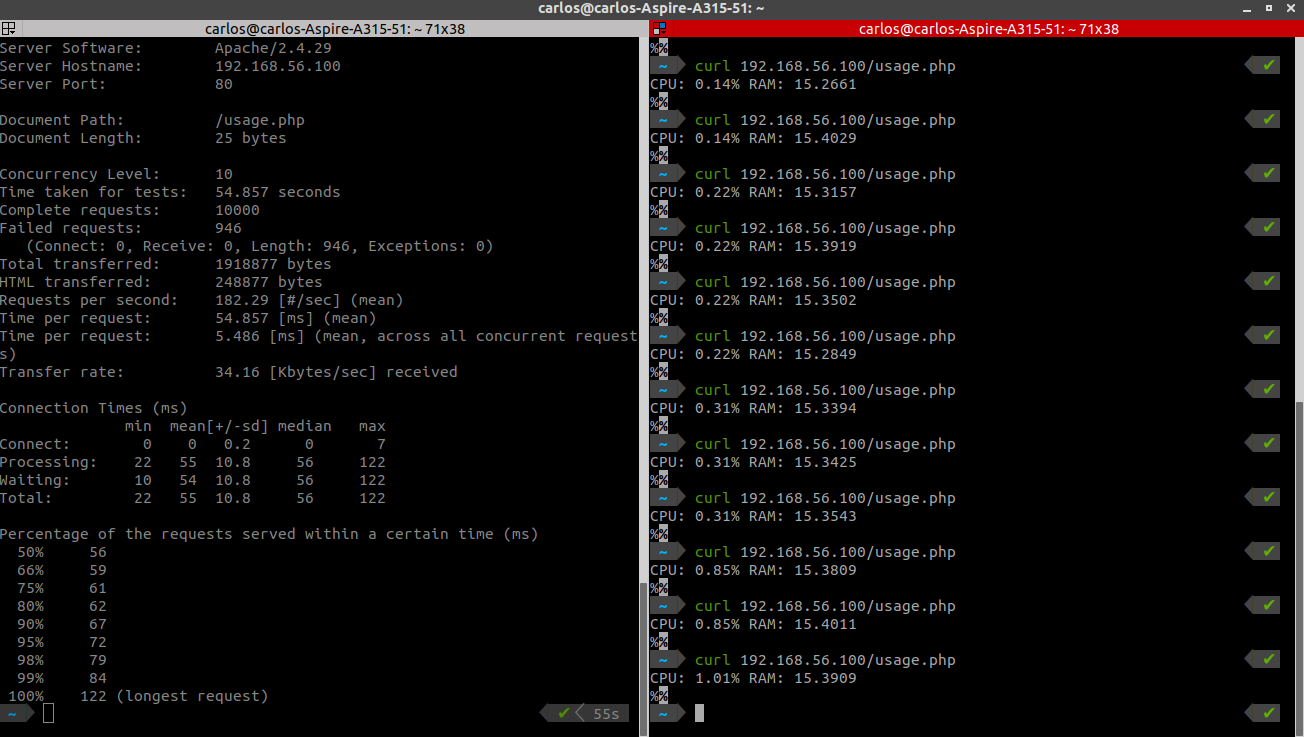
\includegraphics[width=\textwidth]{/t4/usage_ok.png}
	\end{figure}
\end{enumerate}

\end{document}
